\documentclass[a4paper]{article} % set paper size

\usepackage[utf8]{inputenc}
\usepackage {url}
\usepackage[top=2.0cm, bottom=2.0cm, left=2.54cm, right=2.54cm]{geometry} % set margin
\usepackage{amsfonts} % for set names
\usepackage{amsmath} % for equation system
\usepackage{amsthm} % for theorem block
\usepackage{fixltx2e} % for subscript
\usepackage{fancyhdr} % for footer/headline modification
\usepackage{xcolor}
\usepackage{graphicx,float} % for image insertion
\usepackage{multicol} % for text in tow columns

\usepackage{wrapfig} % figure wrapping


\pagestyle{fancyplain} % for footing modification on all pages
\fancyhf{}
%\renewcommand{\headrulewidth}{0pt} % remove decorative lign

\fancyhead[L]{Pauline Maury Laribiere\\
              Alexandre Devienne}
\fancyhead[R]{MT/EL-BA2 EPFL \\
                \today}
\fancyhead[C]{\textbf{Spring programming project : Microcosmos}}

\fancyfoot[R]{\thepage\ of \pageref{lastpage}}

\begin{document}
\begin{multicols*}{2}
% =====================================================================
\section{Architecture and implementation details}

\subsection{Architecture}
\begin{figure}[H]
\centering
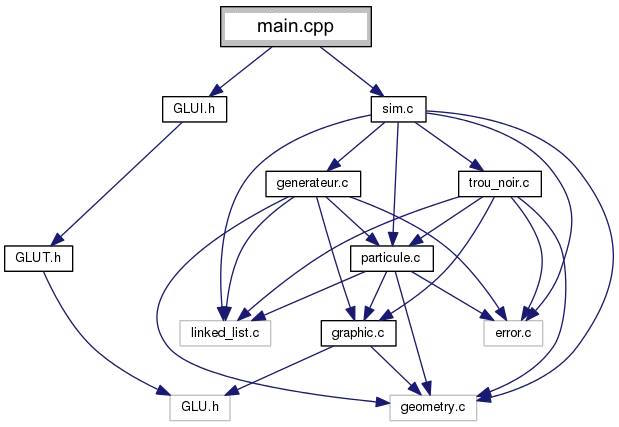
\includegraphics[width=0.48\textwidth]{architecture.jpg}
\caption{Final architecture}
\end{figure}

From rendu 2 to rendu 3, there weren’t any major changes,
we simply finished the coding where and how we had foreseen it.

% Further description of the implementation
% ...

\subsection{Data managment}
To store, manage and delete the data, we used list linked.
Indeed, it was appropriate because the memory could be dynamically handled,
which was necessary for this program.

\subsection{Calculation and memory costs}

\subsection{Illustrations}

% find nice pictures
% ...

% =====================================================================
\section{Methodology}
\subsection{Work organisation}
First of all, even before starting the project,
Alexandre had the idea to use GitHub to work together.
During the whole project, this was a major asset because we could easily share
what we had done with the other without having to send mails
and always check which file had changed and such.
Moreover, it forced us to be rigorous in our way to commit our work
because we had to explain every time which changes had been made.
Before each rendu, we shared the work that had to be done
according the different testing mode of the program.
For the first rendu, one had to do the Error mode and the other the Force mode.
Then, for the second one, there were the Graphic and the Integration mode.
Finally, for the last rendu, we shared the last specifications:
one finished the OPENGL and GLUT
and the other the rest of the whole Simulation mode.
Of course, these shares were not exclusive
and there were still a lot of help between ourselves.

We began the program with the main.cpp and sim.c for the rendu 1.
Very soon, we made the geometry.c module because it eased our work
by reducing the amount of redundant code.
Concerning the testing, first, we always both separately compared each file
with the demo file that had been given to see check that everything looked
and functioned the right way.
Also, other testing file were made in order to check if everything was working right.
The most frequent bug was due to issues with pointers and forgets to initialise correctly datas.
There were also major issues 

% =====================================================================
\subsection{Person responsible for each module} % change to a table in a floatinng figure
\begin{itemize}
\item \texttt{main.cpp}  :  Pauline Maury Laribière
\item \texttt{sim.c :} Alexandre Devienne
\item \texttt{particule.c :} Alexandre Devienne
\item \texttt{générateur.c :} Alexandre Devienne
\item \texttt{trou\_noir.c} : Alexandre Devienne
\item \texttt{list\_linked.c} : Alexandre Devienne
\item \texttt{geometry.c :} Pauline Maury Laribière
\item \texttt{graphic.c :} Pauline Maury Laribière
\end{itemize}

% =====================================================================
\subsection{Auto-evaluation of our work}
To conclude, we can say that we are satisfied with our work.
Even though our programming levels were very different,
we both learned a lot thanks to this project.
We did not used the intermediary rendu to change
but there were very interesting to see another way of coding the same things.
A weak point was the fact that the lessons of the course had to be understood
and handled very quickly to succeed to do the program.
A strong point was the help of the assistants every week.
(je bullshit mais je sais pas quoi metre… )
A possible upgrade would be to have even more exercises in every week’s series
to have the possibility to train ourselves more (BULLSHIT EXTREME ICI AUSSI).

\section{Conclusion}
This project was awesome, we learned all these cool stuf,
but was difficult cause of
still great thanks to all the material YOU gave us

\label{lastpage}
\end{multicols*}
\end{document}
